% Citations should be in bibtex format and go in references.bib
\documentclass[a4paper, 11pt]{article}
\usepackage[top=3cm, bottom=3cm, left = 2cm, right = 2cm]{geometry}
\geometry{a4paper}
\usepackage[utf8]{inputenc}
\usepackage{textcomp}
\usepackage{graphicx}
\usepackage{amsmath,amssymb}
\usepackage{bm}
\usepackage[pdftex,bookmarks,colorlinks,breaklinks]{hyperref}
\hypersetup{linkcolor=black,citecolor=black,filecolor=black,urlcolor=black} % black links, for printed output
\usepackage{rotating} % Rotating table
\usepackage{memhfixc}
\usepackage{pdfsync}
\usepackage{subcaption}
%\usepackage{fancyhdr}
%\pagestyle{fancy}

\title{Human-Computer Interaction Assignment}
\author{Zarif Akib, David Baghumyan, Piet Van Der Paelt and Tibo Vanclooster (Group 3)}
%\date{}

\begin{document}
\maketitle
\tableofcontents
\listoffigures



\section{Introduction}\label{intro}
In the context of the Human-Computer interaction course, taught in the first semester 2Ba computer sciences at the Vrije Universiteit Brussel, students are assigned a group project in which they collaborate to put the acquired knowledge during the theory classes into practice. The assignment that is treated in this report consists of implementing a (mobile) app that allows citizens to get an overview of what is available at the library. Users should also be able to rent materials such as books and movies from the library, and book rooms or computers in advance.\\
\begin{figure}[h]
	\centering
	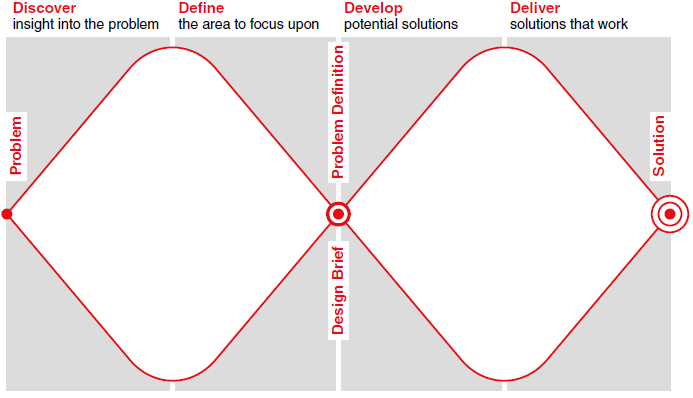
\includegraphics[width=0.6\linewidth]{figures/DoubleDiamond}
	\caption{The double diamond of design\cite{doubleD}}
	\label{fig:doublediamond}
\end{figure}


To accomplish this task, the Double Diamond Design Process was applied. The process is depicted in figure \ref{fig:doublediamond}. The process entails several activities such as discovering requirements, designing alternatives, prototyping and evaluating \cite{sharp2023interaction}. All of these activities come forward in the following sections.

\section{Problem definition}
A first step in the Double Diamond Design Process is to discover the problem. Getting acquainted with the users is essential in this step. The approach taken is to experience the problem ourselves. This initial reconnaissance is follows by the definition of primary, secondary and tertiary users. Having done that, a number of interviews were conducted with users, to be able to create an empathy map. Lastly, Impact mapping allowed us to identify features and requirements that had to be withheld during the development.

\subsection{Empathise: visit to the library}
A very straightforward strategy to empathise, is paying a visit to the library and experience its processes ourselves. The library is what you would expect from any (university) library, but if one starts looking a bit more profoundly, there are some attention points. The library is situated in building C at the Etterbeek campus. There is also a Medical Library at the Jette campus, but that one is out of scope.\\
When arriving at the library, we are confronted with several signs. The sign depicted in figure \ref{fig:affluences} is about the "Affluences" application, but upon arriving at the library it is unclear what is its role. When entering the library there is also a sign directing towards the reading rooms. 

\begin{figure*}[h]
	\centering
	\begin{subfigure}[t]{0.5\textwidth}
		\centering
		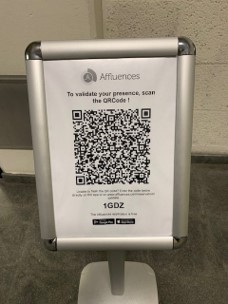
\includegraphics[width=0.5\linewidth]{figures/affluences}
		\caption{Affluences sign}
		\label{fig:affluences}
	\end{subfigure}%
	~ 
	\begin{subfigure}[t]{0.5\textwidth}
		\centering
		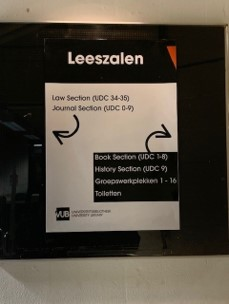
\includegraphics[width=0.5\linewidth]{figures/directions}
		\caption{Directions sign}
		\label{fig:directions}
	\end{subfigure}
	\caption{Signs in the library}
\end{figure*}

From the introduction in section \ref{intro}, we know there is a process that currently allows users to book rooms and computers. It is only after having inspected one of the study/collaboration spots where you can sit down and study it becomes clear the sign in figure \ref{fig:affluences} is actually the application you need to use to reserve a spot and the sign in figure \ref{fig:directions} instructs you where these study/collaboration spots are located.\\

Furthermore, the entrance hall is cluttered with more signs like these. The conclusion would be the user is confronted with lots of information upon arrival. Some of it is relevant, but other information is less relevant upon the first visit. And it is difficult to distinguish between the information that guides you to either renting books or reserving spots, and other secondary services the library has to offer. It would be better to emphasise on the core functionality of the library and hide information that doesn't matter upon arrival.

\subsection{Primary, secondary and tertiary users}
The \textbf{Primary users} of the application consist of broadly speaking any VUB-related person that is involved in academic activities (faculty staff and students). We exclude VUB support staff from this category. Furthermore we distinguish amongst students, researchers, professors (or any teaching staff) and event planners, as far as the event is related to the academic mission of the university. The interest of the student further divides this type of primary user: he/she can be either searching for a certain book, or he/she can be looking for a quiet spot to study\footnote{The library only offers this service in a bookable way during exam periods} or to collaborate with other students on a group assignment. The rationale behind this choice is the definition of the primary user: only the frequent hands-on users should be retained.\\

The \textbf{Secondary Users} consist of the library personnel. Librarians and people managing the library will be confronted with the solution as well, but from a different angle. To fulfil the tasks in the context of their daily activities, it is our estimate they will use other information systems that are already in place it is not our goal to replace these systems. Since our goals are to ease resource access, which is primarily of concern to the primary users in this specific case, we feel the librarians are typically the group of admin users, hence secondary users. They will however assist the primary users when they have questions about the app. We furthermore include external people in this category. These consist of academic staff from other universities and people attending a short course. This group of users typically will be the "guest account" which have limited access and lifetime within the system. They are less frequent users and therefore, fall under the category of secondary users.\\

The last category of \textbf{Tertiary Users} consists of VUB employees in general (all departments), including the support-of-the-support, such as maintenance personnel. 

%\subsection{Context of use}
%maybe address ethical issues here?
%how will risks and benefits will be distributed?
%which impacts van we anticipate?

\subsection{Design goals and requirements}

A number of open-ended interviews (also unstructured interviews) were conducted with students in preparation of establishing an \textbf{Empathy Map Canvas}. During a thematic analysis, common Themes that were identified in these interviews include  reservations of both group collaboration spots (also group work spaces) and individual spaces. It turns out a distinction needs to be made between exam periods and the time outside these exam periods. Outside exam periods, the current reservation system is only active for group collaboration spots. Other resources such as individual spots and computers are not sparse at that time and are not managed. During the exam period the situation changes: all spots need to be reserved prior to usage.\\

The reservation of books and other media is an aspect that didn't appear much during interviews. This aspect doesn't appear to be vivid amongst interviewed students, but it is certainly a core service of the library and is also a hard requirement in the assignment.\\

Since the number of interviews was limited, the analysis could be done manually. The resulting Empathy map is depicted in figure \ref{fig:empathymapcanvasstudents}\\

\begin{figure}[h]
	\centering
	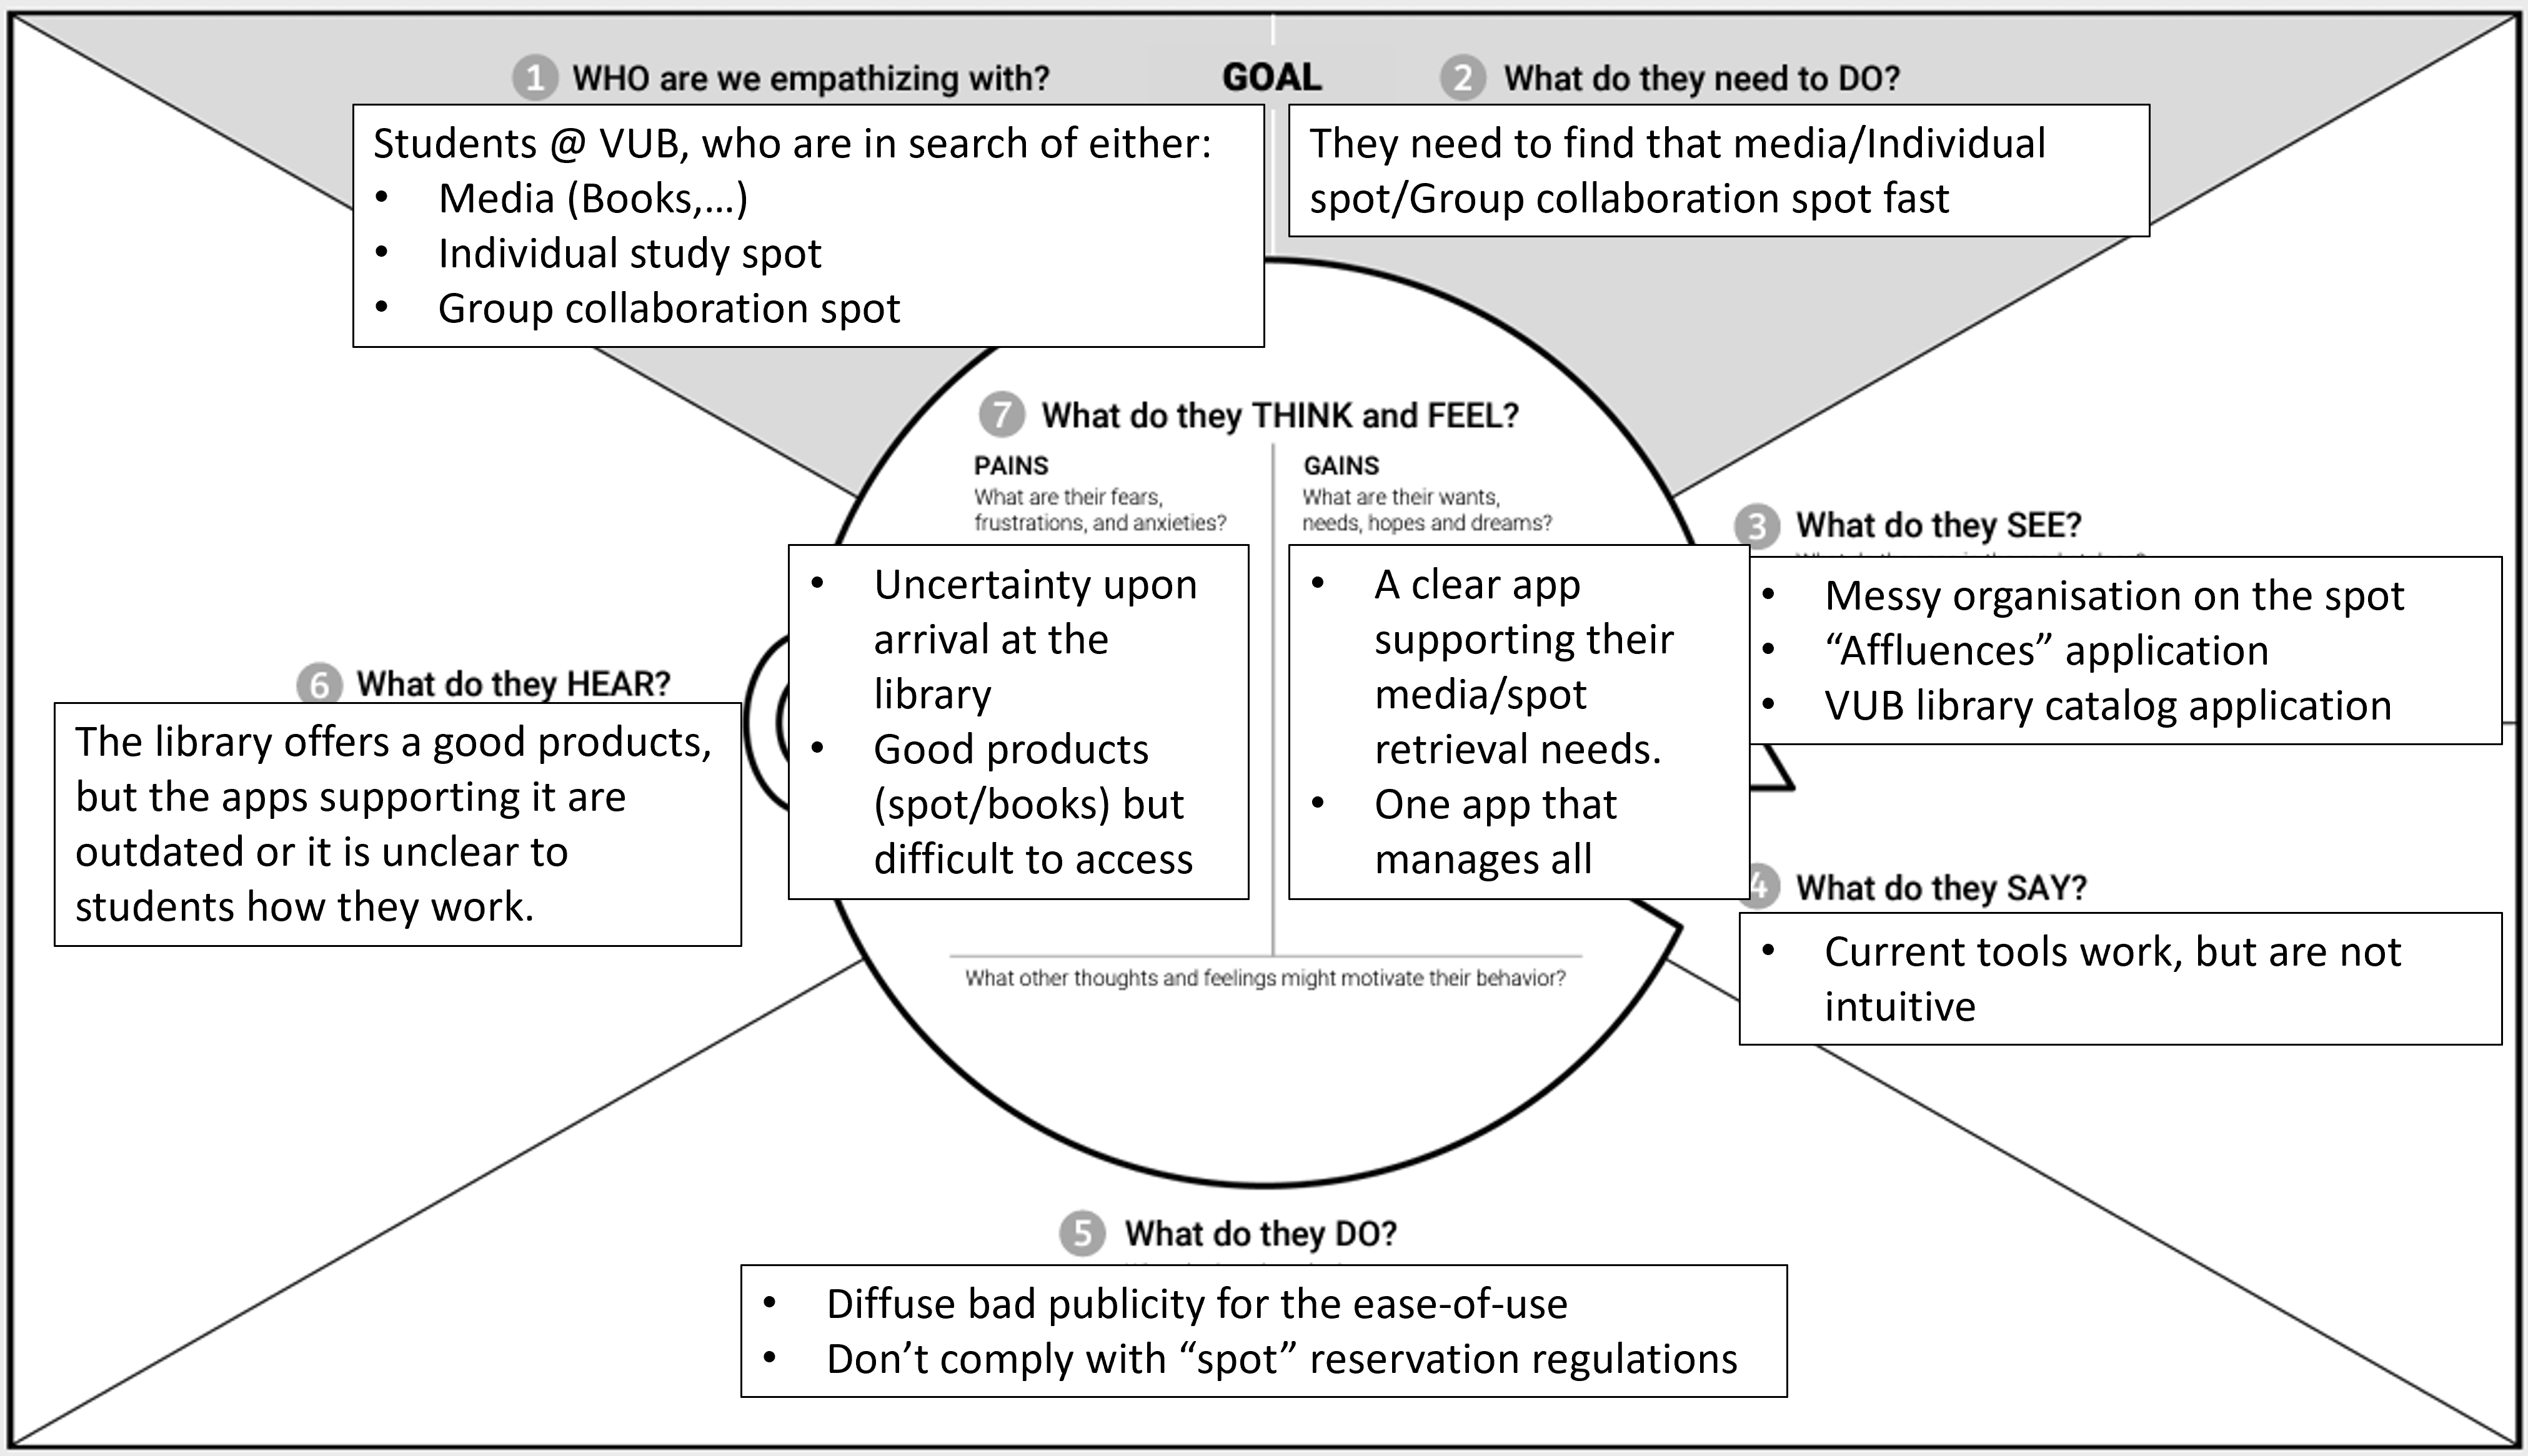
\includegraphics[width=0.8\linewidth]{figures/EmpathyMapCanvasStudents}
	\caption{Students Empathy Map Canvas}
	\label{fig:empathymapcanvasstudents}
\end{figure}

Having completed the Empathy Map for students, a Business Centric Impact Map was created starting off from the business goal to provide individual quiet study spots to students. Through the different stages of the business centric impact mapping, we can identify three goals that need to be achieved: 
\begin{enumerate}
	\item Provide Individual Quiet study spot
	\item Provide Group collaboration spot
	\item Provide access to media
\end{enumerate}
In a commercial setting, all of these would create added value. In this setting, we could quantify each of them as providing a certain utility to the users. That way the attaining the goals contributes to a broader business goal where the library exists in support of the broader academic mission of the university.\\

\begin{figure}[h]
	\centering
	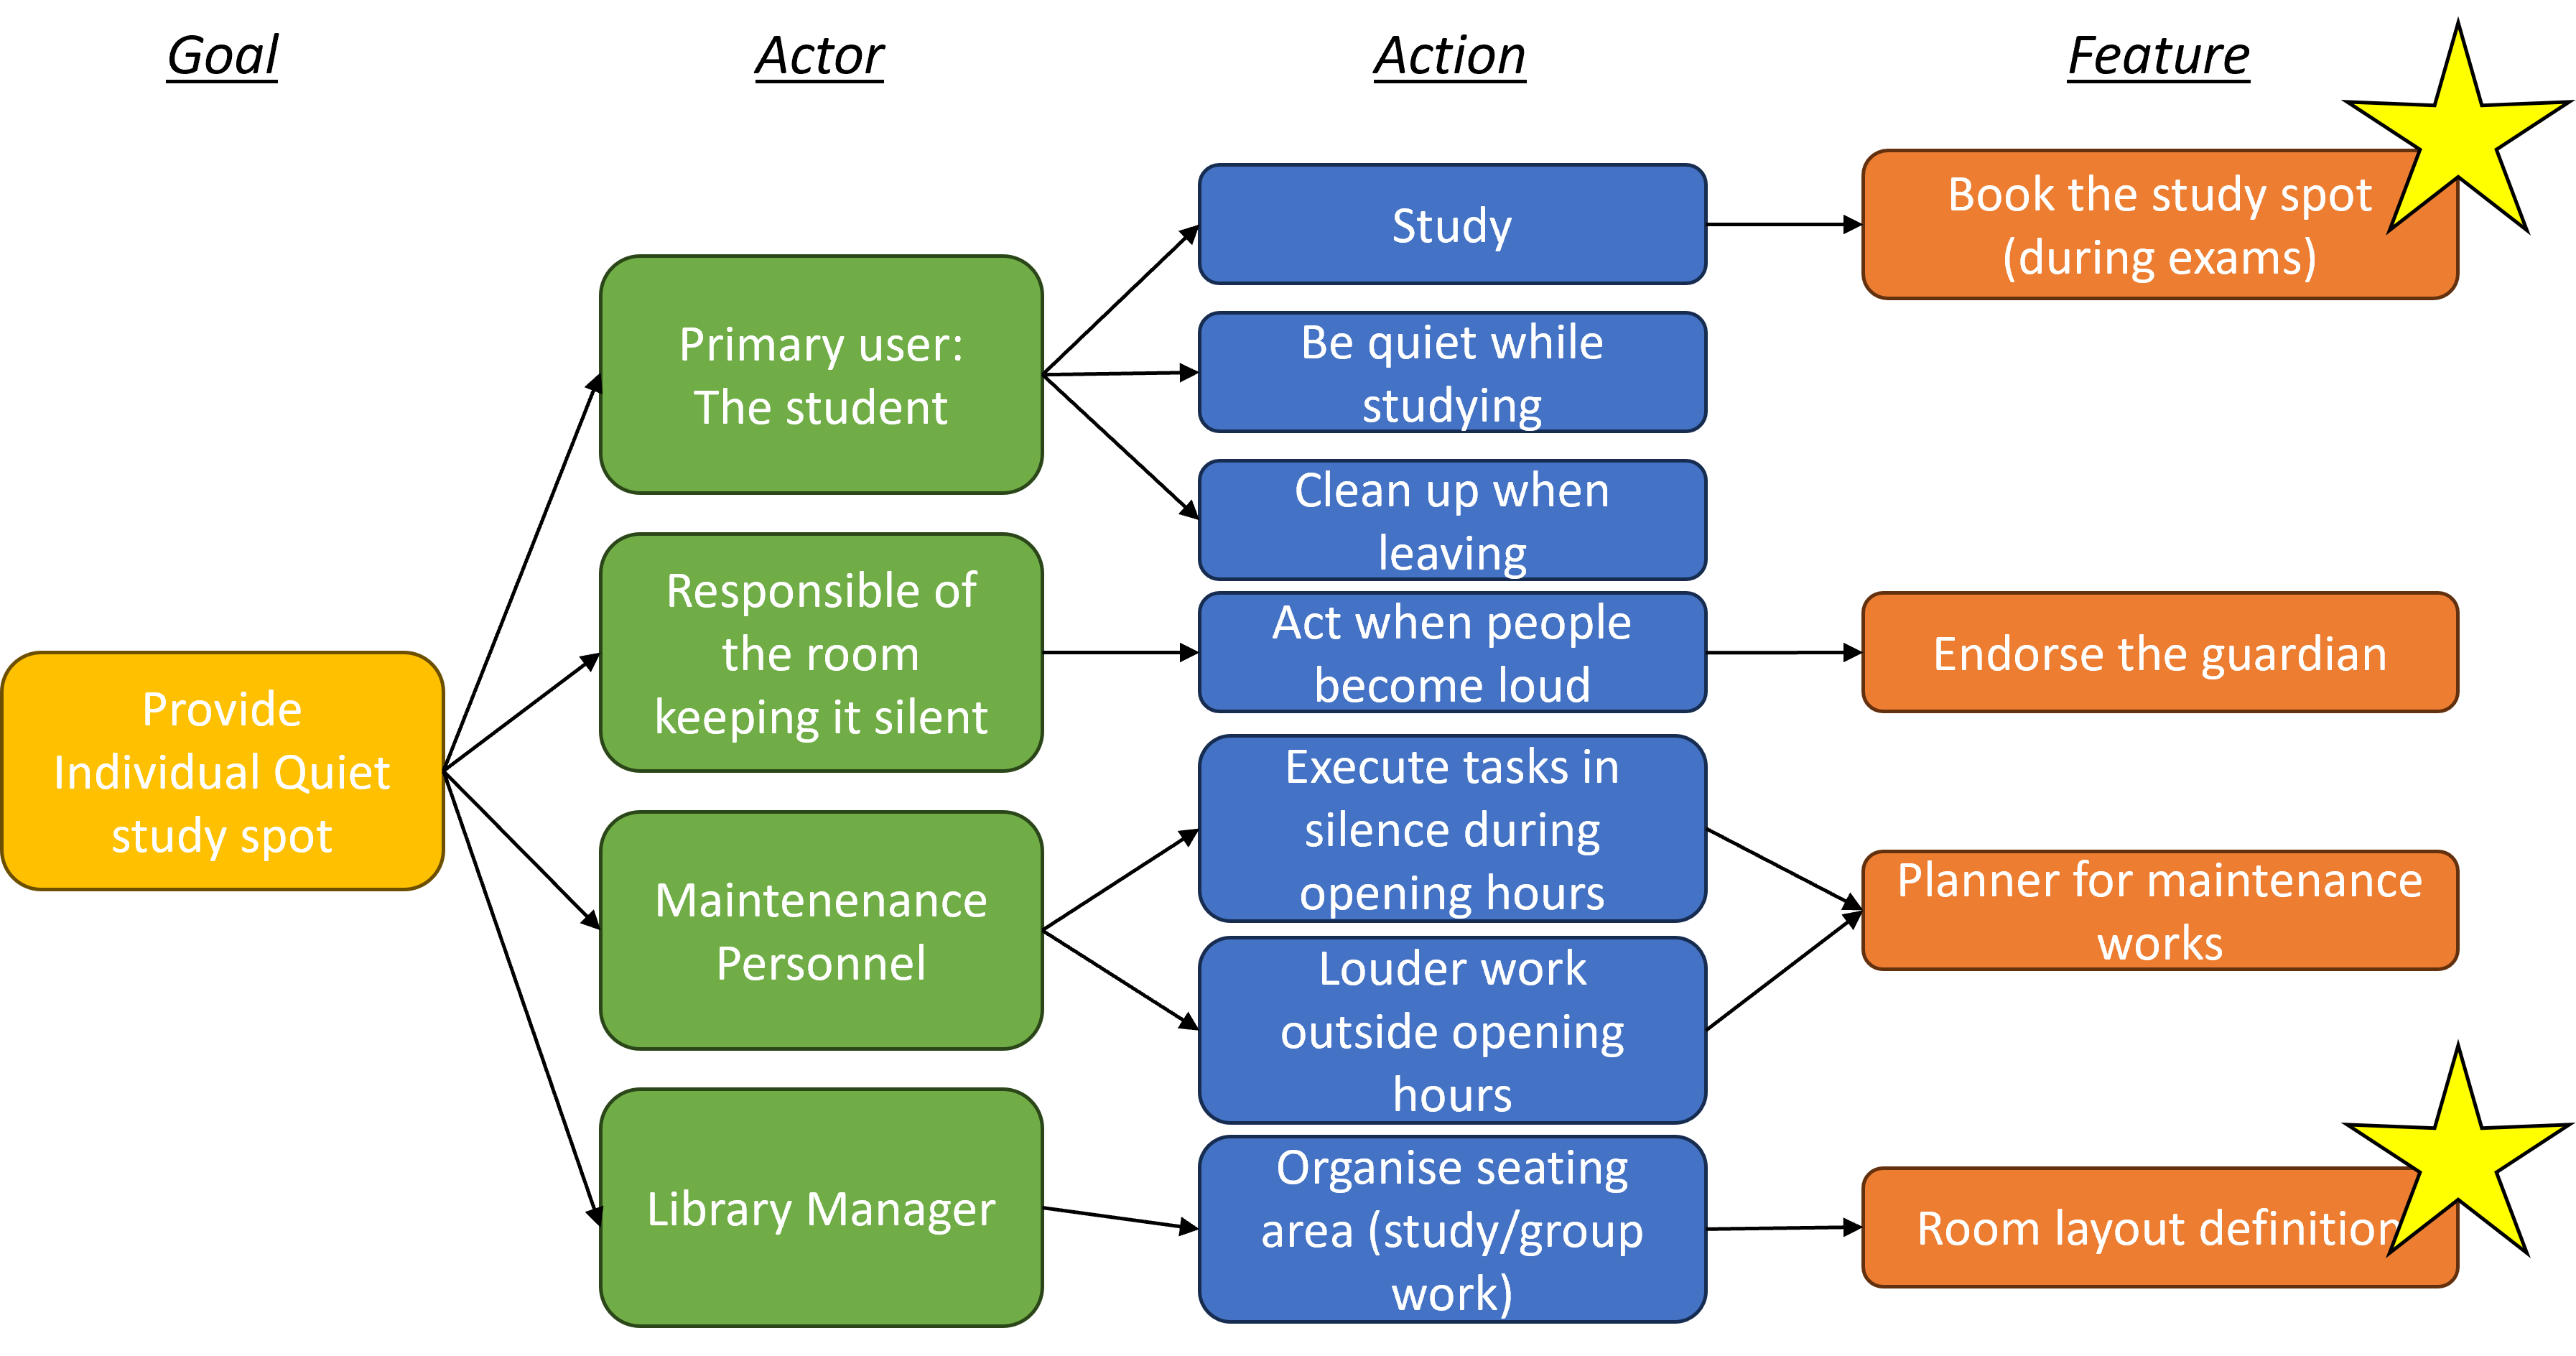
\includegraphics[width=0.7\linewidth]{figures/ImpactMapStudySpot}
	\caption{Business Centric Impact Map: Providing quiet study spots}
	\label{fig:impactmapstudyspot}
\end{figure}

The impact map for the first business goal is depicted in figure \ref{fig:impactmapstudyspot}. The actors that can help to achieve the goal span primary, secondary and tertiary users. All of them can do actions that help to achieve the goal, but in our case, only a few are retained as features that we consider paramount for the final solution, and hence, must certainly be included. It concerns the booking functionality and the room layout definition for easy localisation. \\

The second impact map that is oriented towards the goal to provide collaboration is quite similar to the impact map that treats individual study spots and is therefore not shown. The points where they differ are:
\begin{itemize}
	\item All references to "silent" need to be replaced by "not too loud", since in group collaboration one can expect a certain level of noise to be necessary, and hence must be tolerated
	\item The track along the library manager needs to foresee these spaces in the library so they don't bother the quiet study spots.
\end{itemize}

The third and last impact map is the one where we strive to offer books to the broader public. In this business goal, we encounter the students, librarians and the library manager in the actor role. The primary user is searching for a book which will might result in renting a book. Librarians put the returned books back in a location, and the library manager organises the library. This results in the feature to locate books, and a layout definition. The action of renting a book is not withheld at this stage as an important feature since this would imply an alteration of the business processes as they exist currently. A self-checkout doesn't exist today.
\begin{figure}[h]
	\centering
	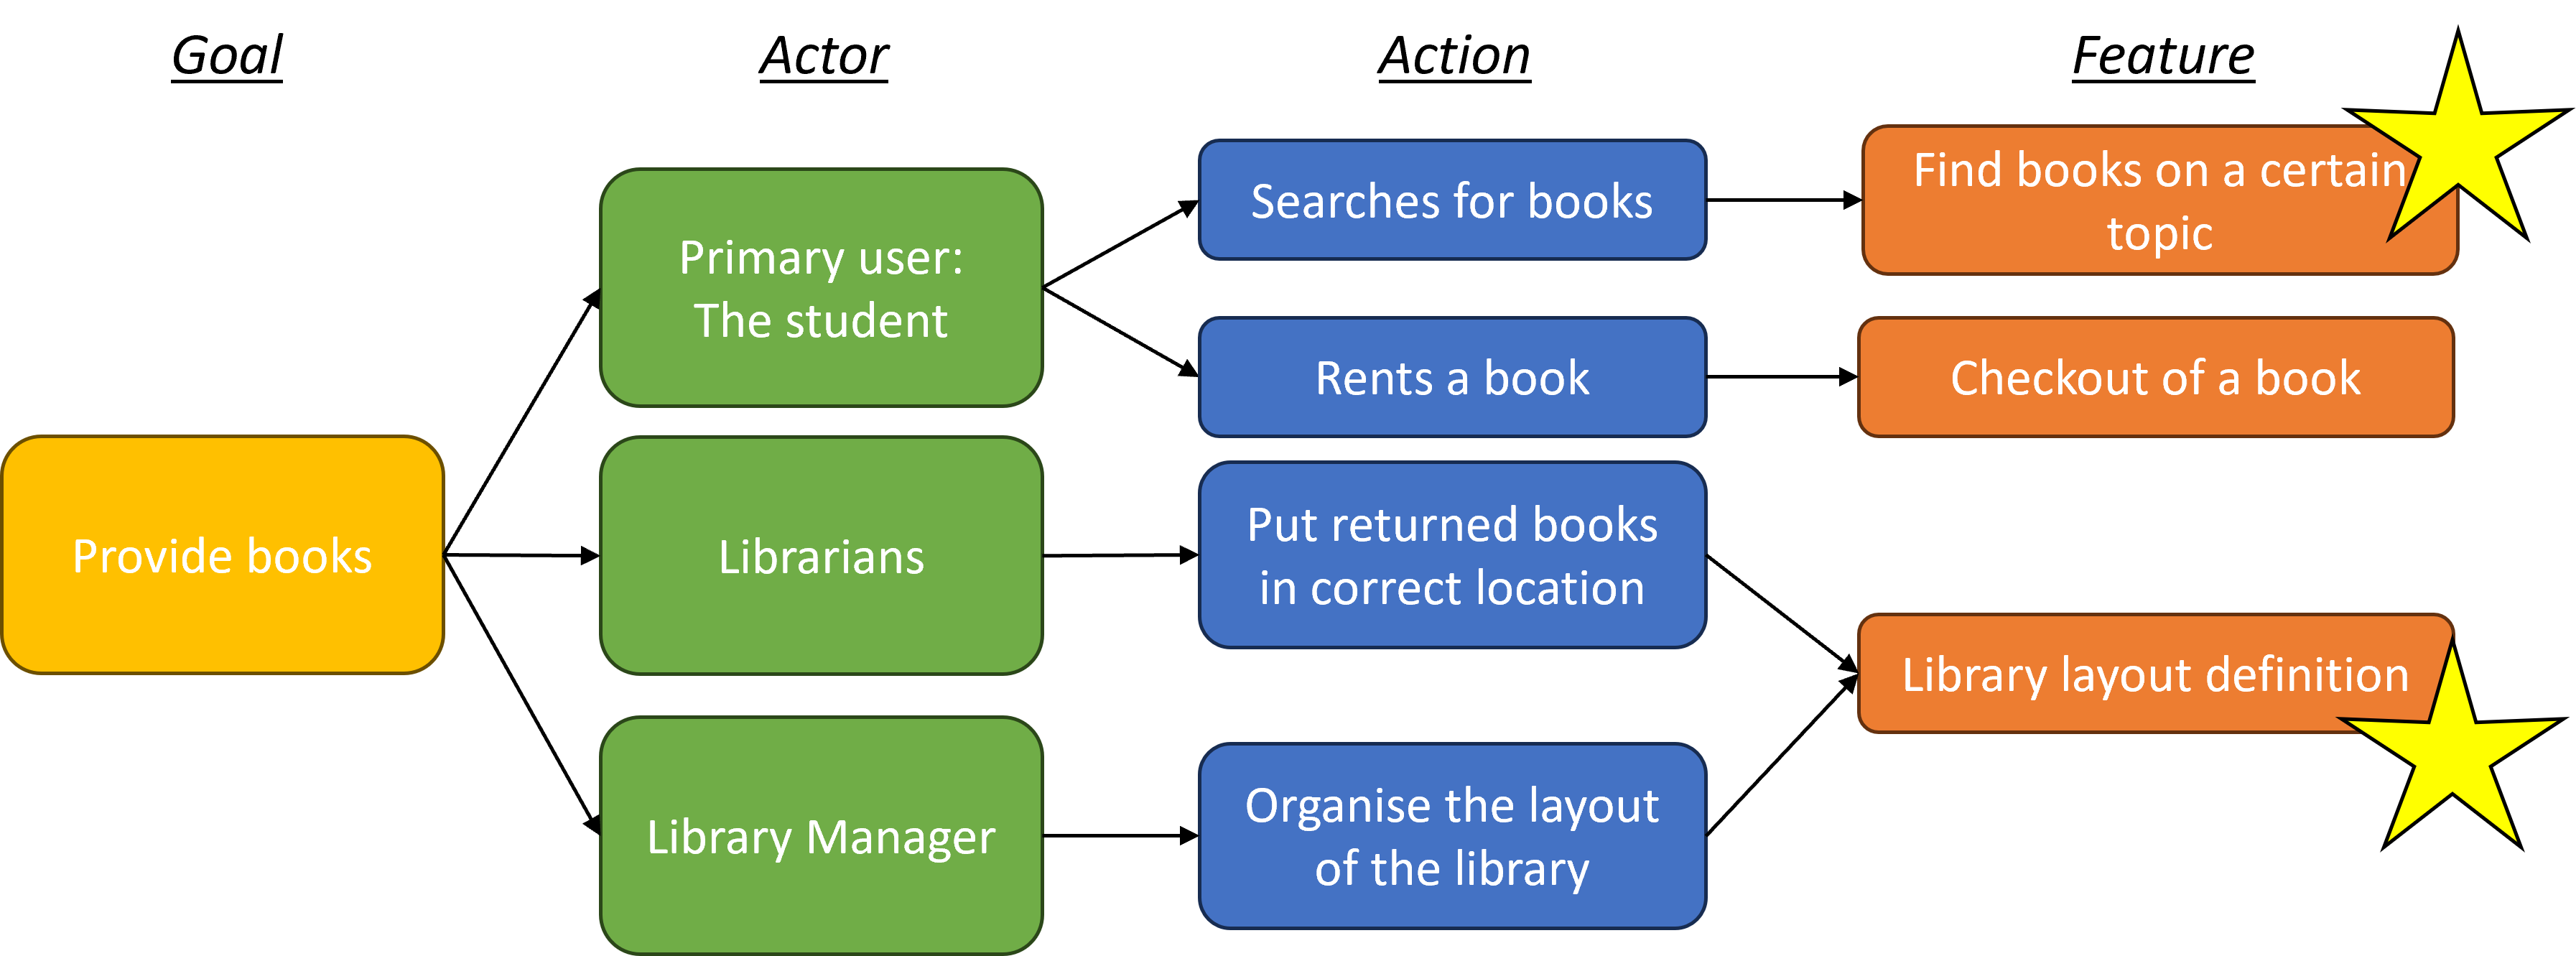
\includegraphics[width=0.7\linewidth]{figures/ImpactMapBook}
	\caption{Business Centric Impact Map: providing books}
	\label{fig:impactmapbook}
\end{figure}
Ultimately, we arrive at the goals the final solution must support. We want to improve the functioning of the library. Find a book must be made easy. The question where every book is located must be answered in a matter of seconds with a visual aid that eases retrieval. Study spots and spaces to collaborate for group assignments must be localizable in the same way, with the same ease. Once a resource is found with the aid of the visual representation of the library, reserving spots (both types) or putting a book on loan which you found in the library must be a straightforward task. Lastly, a Track \& trace functionality for assets must be available as well.\\

Having conducted activities such as empathising, determining types of users and establishing various artefacts (Empathy Maps and Impact Maps), we consider the first phase of the double diamond design process terminated. During the first expansion step, we discovered our target audience, their needs, and the opportunities to contribute to their experience of the library. The "Define" step narrowed this broad scope down to some specific features and goals we desire to support. It concerns the localisation of books, and the two types of spots, and the reservation of the two types of spots. For the books, a direct checkout was not retained, but a waiting list functionality is not in conflict with current business processes and can therefore also be considered as a valid addition to the final solution. From this point on, we are capable of implementing design alternatives in the Develop step, which is the first step in the second phase of the double diamond design process.

\section{Development}
In the development phase, we consider two distinct successive approaches. At first, a low-fidelity prototype was established, which was then evaluated using several testcases during a "Wizard of Oz" experiment. Second, the shortcomings revealed during the evaluation of the low-fidelity prototype where mitigated in the mid-fidelity prototype that was created using the Figma\cite{figma} application\\

\subsection{Low-fidelity prototype}
The development of the low-fidelity prototype started off with the application of the "Crazy-8" method during which the team came up with various ideas to implement the three retained goals. The common ideas were then implemented in a low-fidelity prototype. In our case, we designed several screens that implement the three requirements: 
\begin{enumerate}
	\item Localisation and reservation of books
	\item Reservation of Study spots
	\item Reservation of Group collaboration spaces
\end{enumerate}
\begin{figure}[h]
	\centering
	\includegraphics[width=0.8\linewidth]{figures/lowFid2}
	\caption{Low Fidelity Prototype}
	\label{fig:lowfid}
\end{figure}
The prototype itself was created as a series of 10 cardboard phones with a screen diagonal of approximately 6 inches. This corresponds to the current screen size of contemporary smartphones. Figure \ref{fig:lowfid} shows those 10 cardboard phones in the sequence they will be used to fulfil the goals. The low fidelity prototype allowed to verify the ideas in a more tangible format. Because the approach using cardboard, and primitive representations of concepts in the application, testers felt entitled to give raw feedback, which was useful for further development.\\

Together with the cardboard phones, we established the sequence of screens as they are shown to the end-user. This User Flow is shown in figure \ref{fig:lowfiduserflow}. The screens were numbered (shown in figure \ref{fig:wizoz}) and correspond to the numbers in the user-flow diagram. Most of the arrows linking the screens are bi-directional, due to the need to return from one screen to the previous.\\
In general, the low-fidelity prototype implements currently 2 workflows:
\begin{enumerate}
	\item Localisation and reservation of books: 1-2-5-6-7 and 1-2-5-6-4/8 respectively 
	\item Reservation of Study spots: 1-2-9-7/8
\end{enumerate}
The reservation of group collaboration spaces is currently not implemented in the low-fidelity prototype as it is merely a duplicate of the workflow for individual study spots. The difference is how the spots are used and where they are located in the library.
\begin{figure}[h]
	\centering
	
\includegraphics[width=\linewidth]{figures/LowFidUserFlow}
	\caption{Low-fidelity User Flow}
	\label{fig:lowfiduserflow}
\end{figure}
\begin{figure}[h]
	\centering
	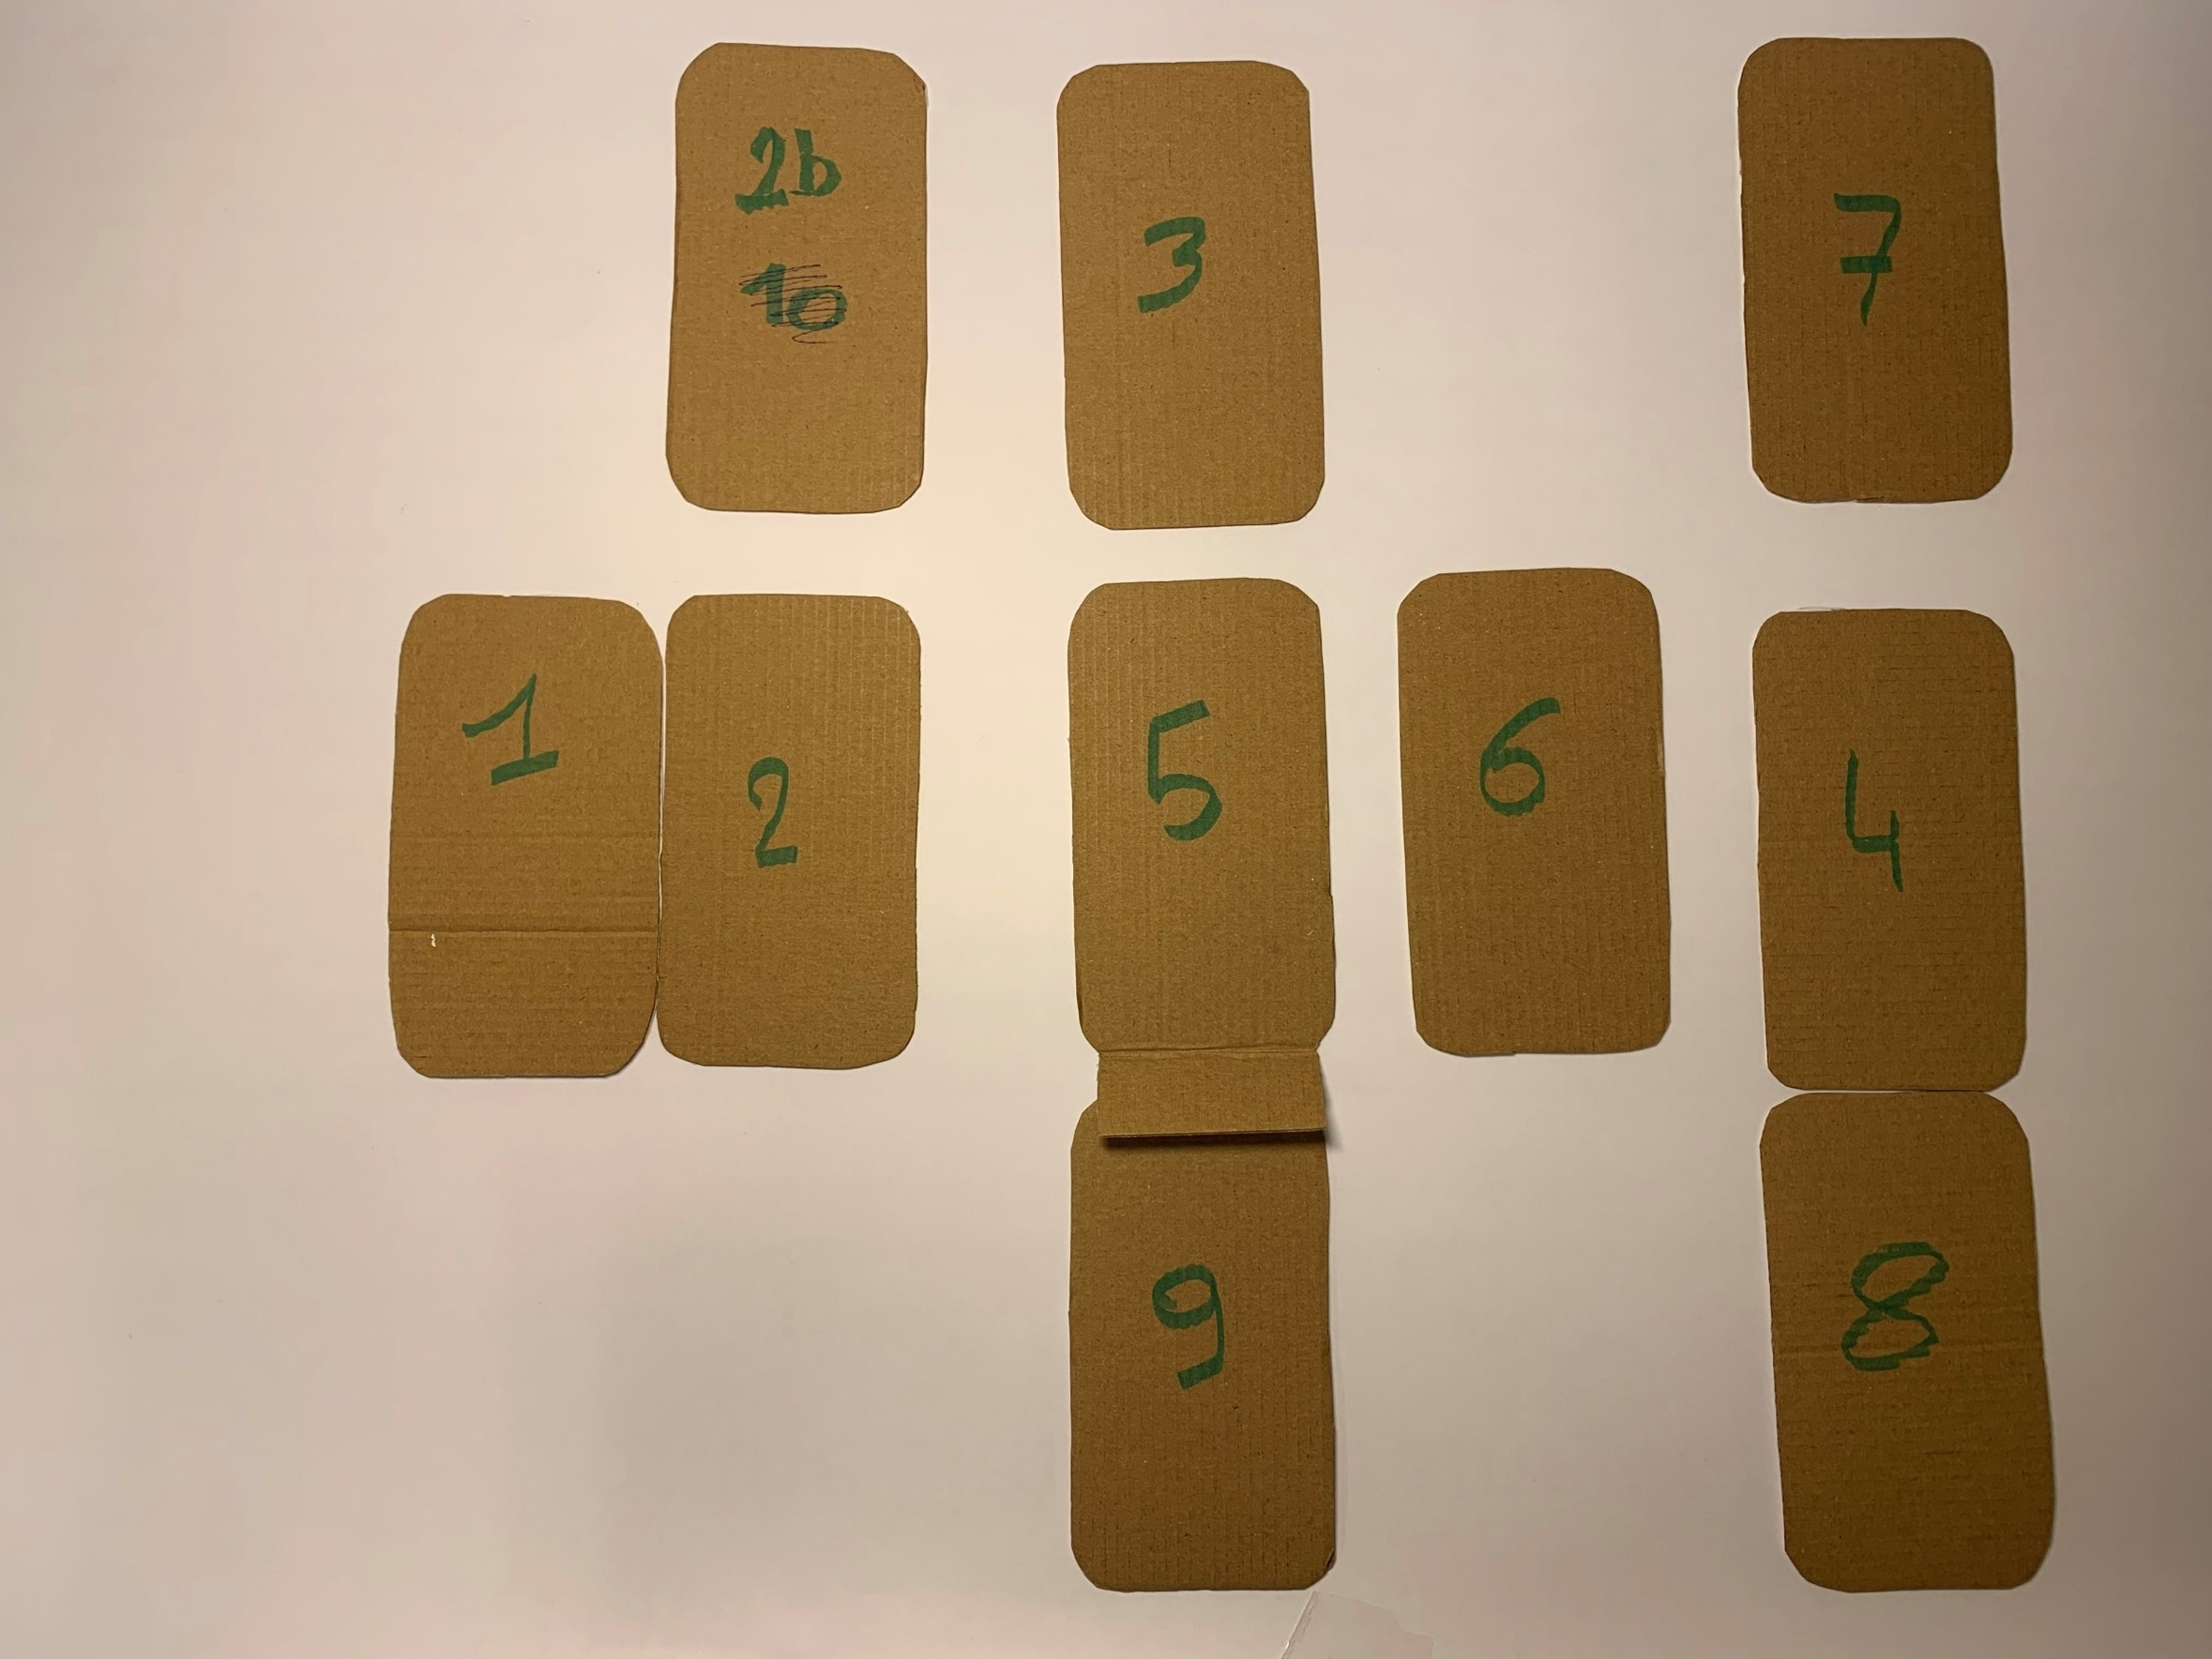
\includegraphics[width=0.6\linewidth]{figures/WizOz}
	\caption{Preparing for the Wizard of Oz experiment}
	\label{fig:wizoz}
\end{figure}
Having completed the user flow, several test-cases were established covering various topics. These include login, verification of current reservations, cancel current reservations and queries for books. The scenarios are shown in table \ref{tbl:testcase}, which is available in appendix \ref{app:tc}. Each scenario includes a task, the screens involved, user action and the resulting app behaviour.\\

The tests revealed shortcomings in the initial low-fidelity prototype such as the inability to return from any screen to the previous. In the low-fidelity prototype such a shortcoming is easily mitigated by drawing a back button on the screen. The tests can be adapted easily and continued with the same user.

\newpage
\subsection{Final Solution (mid-fidelity prototype)}
Having conducted the necessary experiments using the low-fidelity prototype, a mid-fidelity prototype was established using the Figma \cite{figma} application. Figure \ref{fig:figmaOverview} shows the overview of the finalised application. The experiences and remarks from the testing using the low-fidelity prototype were taken into account when implementing this prototype. In that way, the mid-fidelity prototype was prepared for evaluation by a broader and more generic public.
\begin{figure}[h]
	\centering
	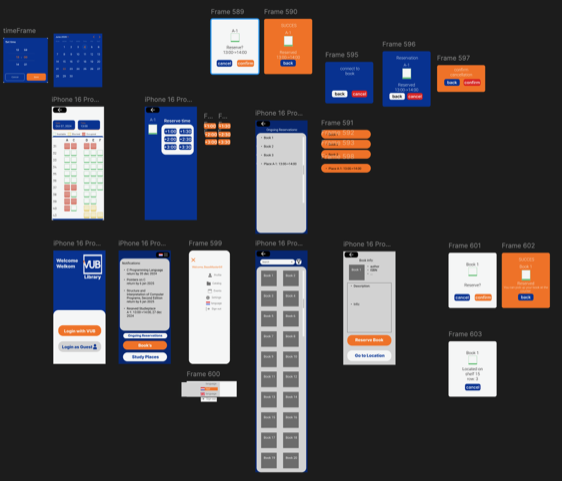
\includegraphics[width=1.0\linewidth]{figures/FigmaOverview}
	\caption{Mid-fidelity prototype application overview}
	\label{fig:figmaOverview}
\end{figure}
\newpage
\section{Evaluation (UEQ+)}
A final evaluation using the Modular Extension of the User Experience Questionnaire (UEQ+)\cite{ueq} was conducted. User testing was done by assigning the user a task in the application. Testers had to reserve an individual study spot, so the intended flow in the application was determined upfront. This flow is depicted in figure \ref{fig:figma}
\begin{figure}[h]
	\centering
	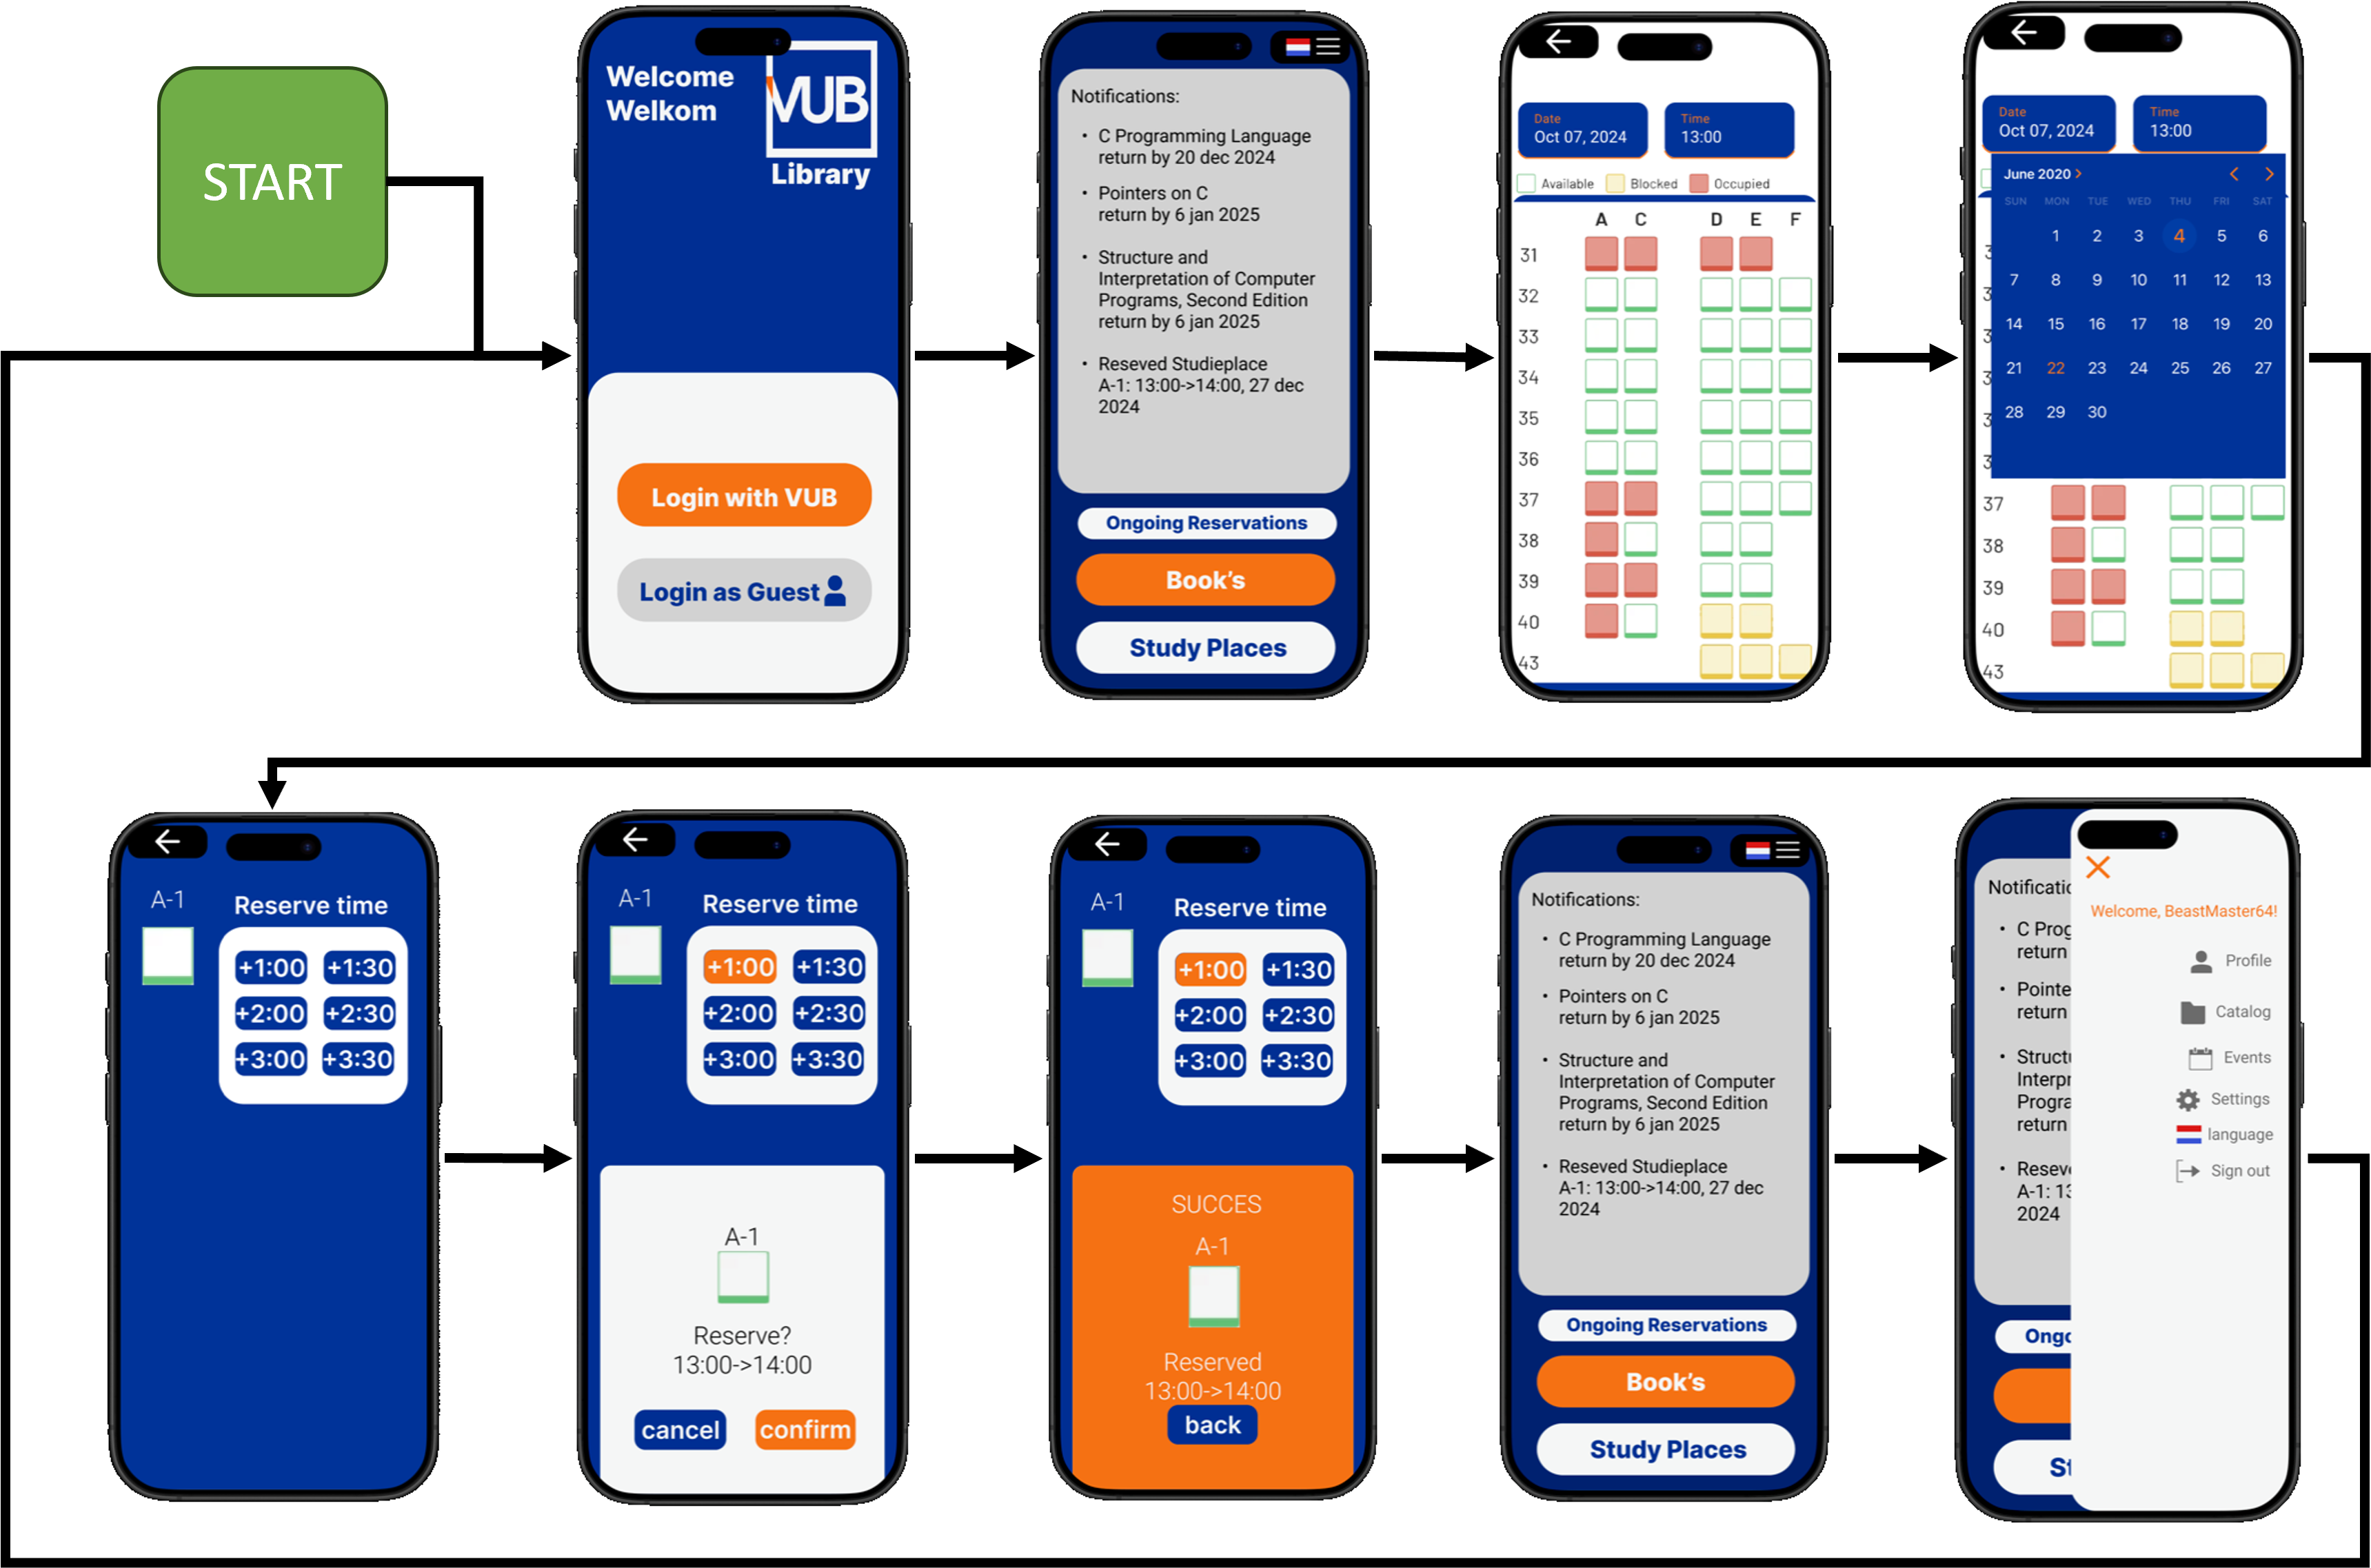
\includegraphics[width=1.0\linewidth]{figures/FigmaReserveSpot}
	\caption{Mid-fidelity prototype study spot reservation flow}
	\label{fig:figma}
\end{figure}
Once the users were ready and had successfully completed the task, either with some help or without help, they were asked to fill out a short survey using the UEQ+ template. That survey included the user experience scales \textbf{Usefulness} (impression that using the product is beneficial), \textbf{Intuitive Use} (impression that the product can be used immediately without any training or help) and \textbf{Clarity} (perception that the user interface is well-structured and of low visual complexity). All of them are implemented on a 1-7 Likert scale, 1 being the lowest score, 7 being the highest score. We limited the choice to three to keep our users motivated. Users also have to assign an overall importance rating to each user experience scale. The Choice of user experience scales was highly inspired to have feedback whether the application was really a valuable addition when compared to existing tools, whether it was easy to use in the sense of "install and use straight away" and clear so no confusion in the interface would be present.\\

The responses were gathered in the VUB community, but due to time limitations, relatives were asked as well to test the app and provide answers to the query. That way, we reached a response for $n = 13$ persons. The data was entered in the analysis sheet, provided along with the other UEQ+ resources.\\

\begin{figure*}[h]
	\centering
	\begin{subfigure}[t]{0.5\textwidth}
		\centering
		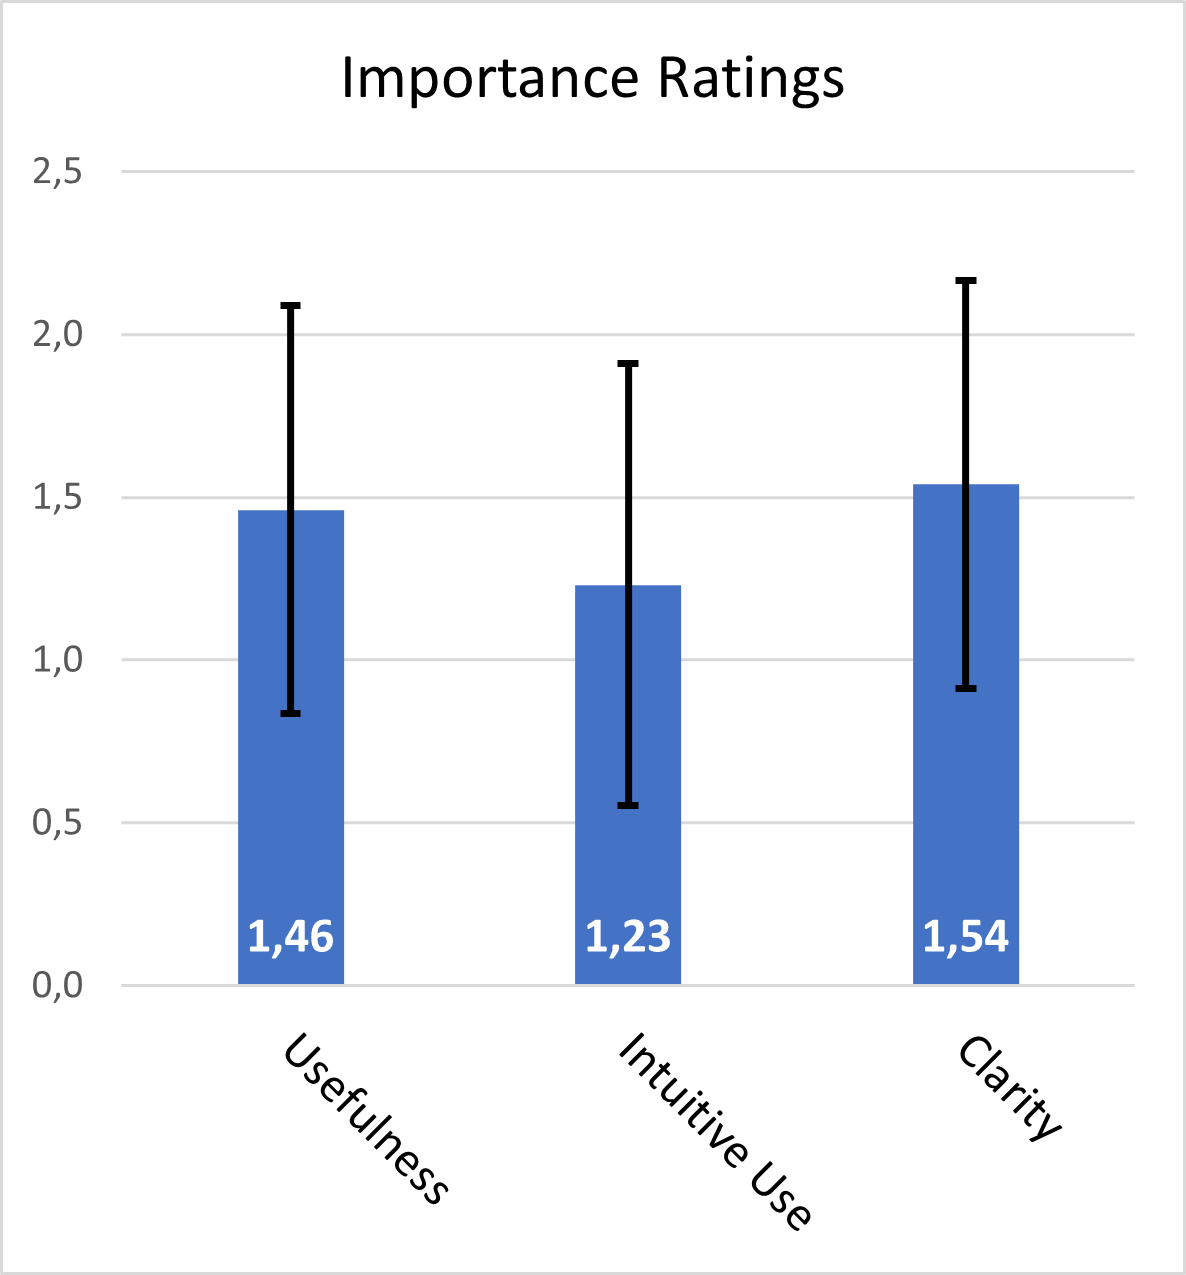
\includegraphics[width=0.7\linewidth]{figures/ImportanceRatings}
		\caption{Importance Ratings Confidence intervals($\alpha = 0.05$)}
		\label{fig:ImportanceRatings}
	\end{subfigure}%
	~ 
	\begin{subfigure}[t]{0.5\textwidth}
		\centering
		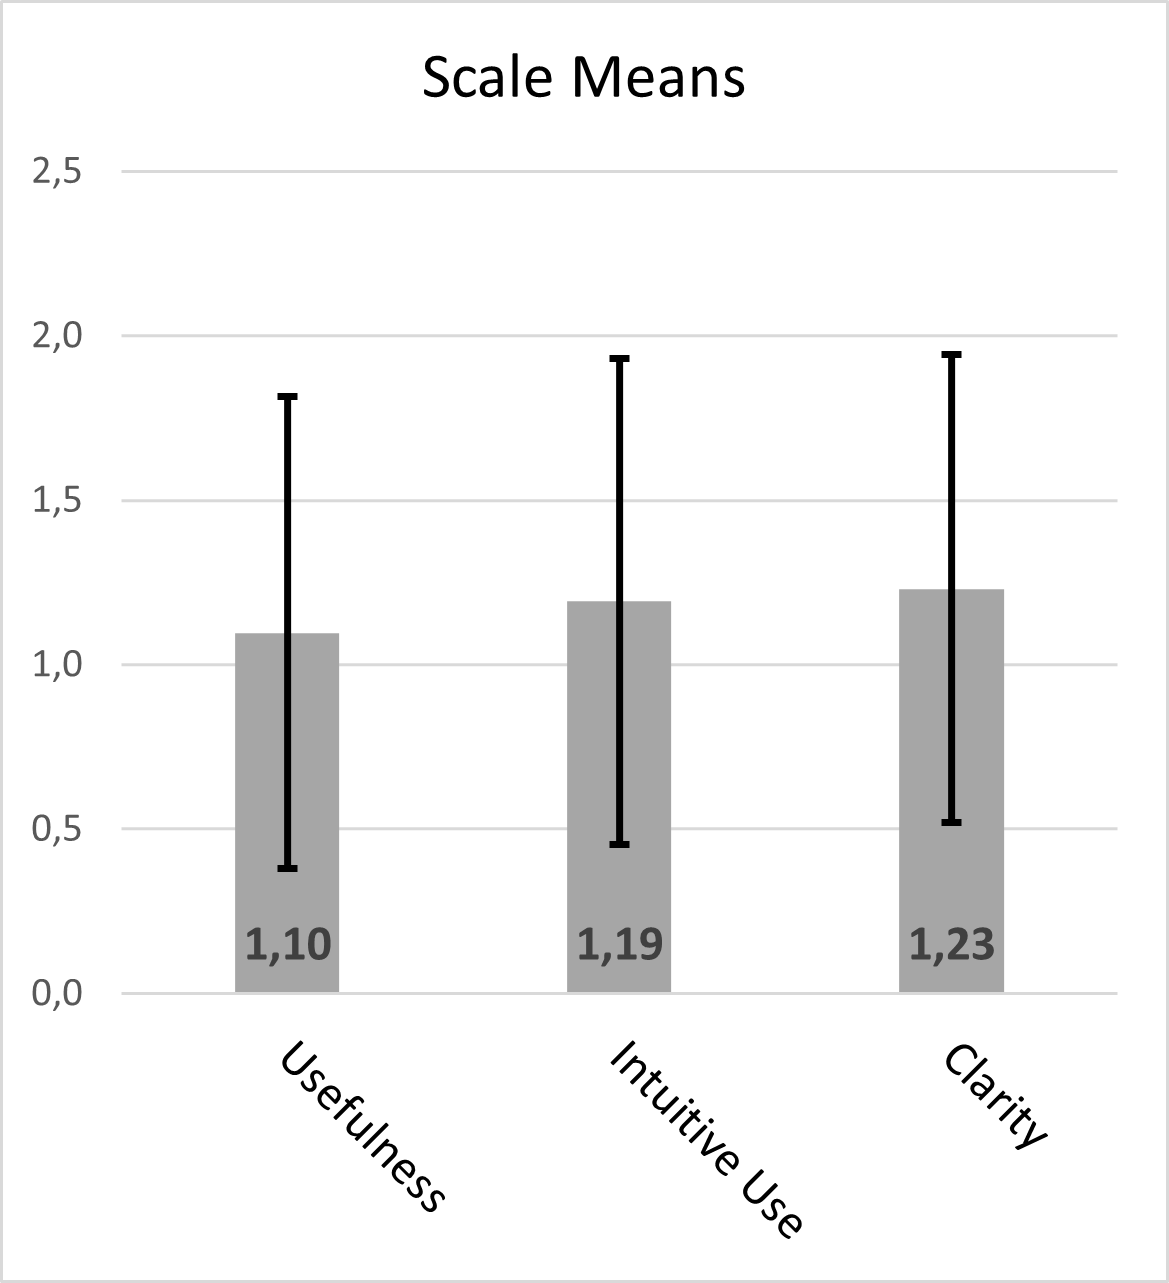
\includegraphics[width=0.7\linewidth]{figures/ScaleMeans}
		\caption{Scale Confidence intervals ($\alpha = 0.05$)}
		\label{fig:ScaleMeans}
	\end{subfigure}
	\caption{Confidence intervals}
	\label{fig:confInt}
\end{figure*}

Figure \ref{fig:confInt} shows confidence intervals for the three user experience scales. The bars represent the mean value, the whiskers (full length) show the width of a 95\% confidence interval. We refer to appendix \ref{app:anova} figure \ref{fig:confint} for the values of the bounds of these confidence intervals. In appendix \ref{app:anova} we also included figure \ref{fig:boxplot} which shows the quartiles and means in a convenient way to compare them. From this image we conclude there is a very limited amount of outliers (2 measurements for the full dataset) which we chose to ignore. The confidence interval is computed using the formula 
\[
	\overline{y} \pm z_{\frac{\alpha}{2}}\cdot \dfrac{\sigma}{\sqrt{n}}
\]
and is implemented in the excel sheet using the function \texttt{CONFIDENCE}, which calculates the half-width of the confidence interval $z_{\frac{\alpha}{2}}\cdot \dfrac{\sigma}{\sqrt{n}}$, assuming a normal distribution.  Means are computed using the \texttt{AVERAGE} function, and from this result a value of 4 is subtracted. This way, the scale undergoes a translation from the $[1,7]$ interval to the $[-3,3]$ interval.\\

When analysing the results for the Ux scale means, we conclude by means of an ANOVA test for the equality of the means the means for the three Ux Scales don't differ (p = 0.87 ). A Browne-Forsythe-Levene test for the equality of variances accepts this equality of the variances (p = 0.82). This confirms the intuition about the equality of the means and variances as a result of the graph's interpretation. For what concerns the importance of the Ux scales, we conclude the means are equal at p = 0.80, using an ANOVA test. A Browne-Forsythe-Levene test for the equality of variances accepts this equality of the variances (p = 0.96). The details of these hypothesis tests are provided in appendix \ref{app:anova}\\

From this analysis we conclude the scales were not rated significantly different by the testers. Furthermore, since the confidence intervals don't include the midpoint of the likert scales, for each User Experience scale the mid-fidelity prototype scores above the midpoint of the scale. The interpretation of such a confidence interval is that we are 95\% sure the real average value for the Ux scale will be between the lower and upper bound. There is however a nuance to that: it concerns a 95\% confidence interval so there must be some accounting for coincidence: there is a chance of 5\% that the real population mean value for the Ux scales is outside these bounds, or in other words 2.5\%of chance the value will be below the lower bound. That however, is a one-tailed interpretation of a two-tailed inference method, and should be avoided. If we were to draw such a conclusion, a one-tailed hypothesis test were we would state $H_a:\mu_{UxScale} > scaleMidpoint$ would be more appropriate.

\newpage
\section{Discussion and Conclusion}

By applying the double diamond design process, we went through the phases of discovery of the problem, followed by the definition of goals and requirements. In this first "diamond", several artefacts led to a better understanding of the users and their needs. Once the promblem statement was clearly defined, we implemented prototypes. Starting off from a low-fidelity prototype, which allowed for fast implementation and user feedback, we implemented a mid-fidelity prototype which was furtherly evaluated using the UEQ+ framework. The combination of prototyping and evaluation constitutes the second "diamond". The resulting prototype covers user needs as proven by the UEQ+ framework assisted evaluation. The average scores for Usefulness, Intuitive use and Clarity confirm this. However, we need to report on the length of the sample we used to obtain these conclusions. Only 13 testers were included and that might be too few.\\

For what is concerned the interviews we conducted, only students were included. Given the scope of primary users, this is a shortcoming since we also should have included academic staff in our primary users group. If this application is to evolve to a full-fledged production application to be used by the entire academic community, these users should be included in another round of UEQ+ testing. From there on, more thorough modifications of the mid-fidelity prototype might be required.\\

Furthermore, during the testing Low fidelity prototype: there were no back-buttons since on android phones you don't need them. On iPhone it is necessary to have them. Such a shortcoming is typically platform-dependent, since on iPhones you need such a button, and on Android devices it can be omitted since that button is inherently part of the operating system. That reveals the shortcoming the app was conceived bearing only iPhones in mind. That is a potential danger since we might miss half of the users.\\

On the statistical analysis using the UEQ+ tools, we have some thoughts regarding the methods applied in the template. These are definitely fine if one is using rather big sample sizes, but in our case we must be cautious on the conclusions drawn. For example: the computation of the confidence intervals in the UEQ+ analysis template makes a rather strong assumption about normality to  compute these confidence intervals. For the applied techniques to be used legitimately, that normality has to be proven if the length of the sample is smaller than $n = 30$ for the central limit theorem for the means to hold. Furthermore, the used formula involving $z_{\frac{\alpha}{2}}$ also assumes the computed standard deviation is equal to the population standard deviation, which is rather a strong assumption given the length of the sample only includes 13 responses. A choice for a t-distribution in the case of unknown population variances and relatively small sample sizes would have been more appropriate. The differences these alterations would imply are not executed. Furthermore the Excel template uses \texttt{STDEV.P} rather than \texttt{STDEV.S}, which is more appropriate in this context. All of these reservations fade away once the sample size gets bigger, i.e. when the t-distribution converges to the N-distribution.\\

\newpage
\appendix
\section{Test Cases}\label{app:tc}
\begin{table}[h!]
	\centering
	\small
	\rotatebox{90}{ \begin{tabular}{|l|l|l|l|}
		\hline
		Tasks & Screen & User Action & App Behavior \\ 
		\hline
		Login: enter email & 1: Welcome screen & Tap "enter email" field & Keyboard slides up \\ 
		\hline
		Enter email & 1 + keyboard slider & Typing name + "done" & Keyboard disappears \\ 
		\hline
		Login: enter password & 1: Welcome screen & Tap "enter password" field & Keyboard slides up \\ 
		\hline
		Enter password & 1 + keyboard slider & Typing name + "done" & Keyboard disappears \\ 
		\hline
		Perform actual login & 1: Welcome screen & Tap login button & Go to screen 2 \\ 
		\hline
		Check all ongoing reservations & 2: Start & Tap "ongoing reservations" button & Go to screen 3 \\ 
		\hline
		Check details of one reservation & 3: Ongoing Reservations & Tap a row & Go to popup 4 \\ 
		\hline
		Close popup 4 & 4: Popup "Res. Successful" & Tap "close cross" & Go to screen 3 \\ 
		\hline
		Check all ongoing reservations & 2: Start & Tap "ongoing reservations" button & Go to screen 3 \\ 
		\hline
		Check details of one reservation & 3: Ongoing Reservations & Tap a row & Go to popup 4 \\ 
		\hline
		Cancel this reservation & 4: Popup "Res. Successful" & Tap "cancel" & Go to screen 3 \\ 
		\hline
		Search for a book & 2: Start & Tap "books" to open screen 5 & Go to screen 5\\ 
		\hline
		Search a title/author & 5: Book Search & Tap search bar & Keyboard slides up \\ 
		\hline
		Enter title/author/... & 5 + keyboard slider & Typing + "done" & Keyboard disappears\\ 
		\hline
		Select a title & 5: Book Search (Filtered) & Tap a tile (represents a book) & Go to screen 6\\ 
		\hline
		Return to filtered books & 6: Book Info & Tap "close cross" to close screen 6 & Go to screen 5\\ 
		\hline
	\end{tabular}}
	\caption{Wizard of Oz experiment Test Cases}
	\label{tbl:testcase}
\end{table}
\newpage
\section{Additional Statistical Analysis}\label{app:anova}
\begin{figure}[h!]
	\centering
	\includegraphics[width=0.7\linewidth]{figures/confint}
	\caption{Confidence interval bounds for Ux scales and Importance}
	\label{fig:confint}
\end{figure}
\begin{figure}[h!]
	\centering
	\includegraphics[width=0.8\linewidth]{figures/boxplot}
	\caption{Box Plots for 12 included Likert scales}
	\label{fig:boxplot}
\end{figure}
\newpage
\begin{figure}[h!]
	\centering
	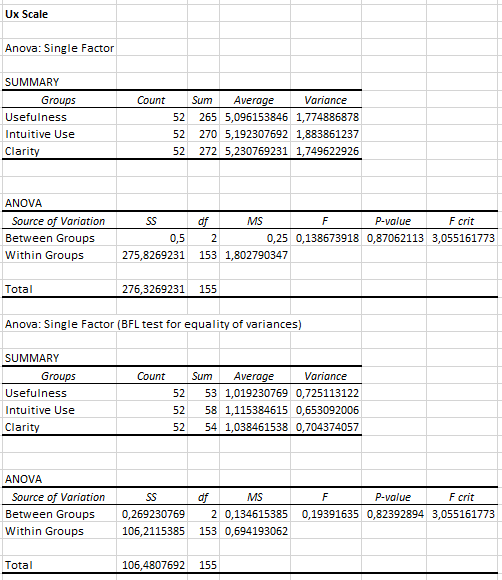
\includegraphics[width=0.7\linewidth]{figures/UxScale}
	\caption{User Experience Mean and Variance analysis for 3 included scales}
	\label{fig:uxscale}
\end{figure}
\newpage
\begin{figure}[h!]
	\centering
	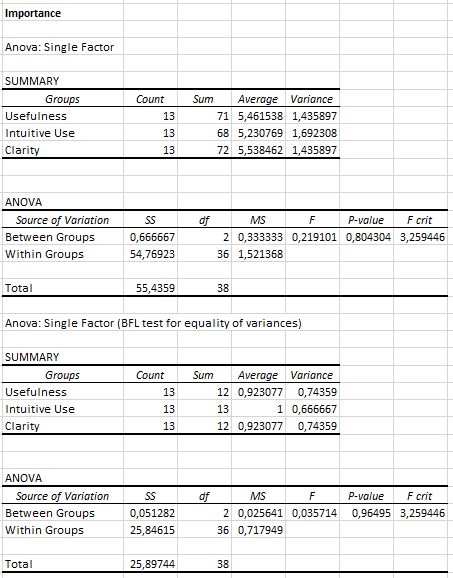
\includegraphics[width=0.7\linewidth]{figures/importance}
	\caption{Importance Mean and Variance analysis for 3 included scales}
	\label{fig:impo}
\end{figure}
\newpage
\bibliography{references}  % need to put bibtex references in references.bib
\end{document}